%\documentclass{article}
%\usepackage{graphicx,subfigure}
%\begin{document}

\begin{figure}[!h]
  \centering
  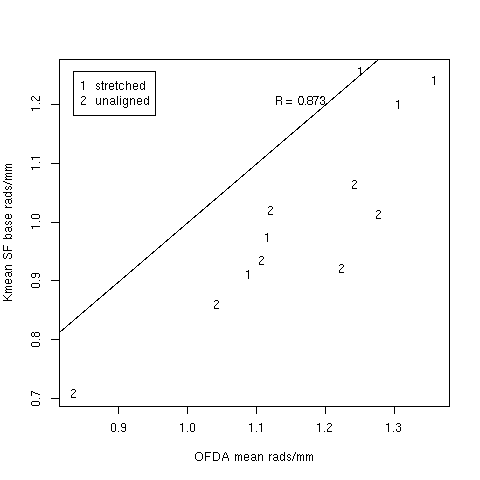
\includegraphics[width=1.0\textwidth]{figofdasimsfbasemean.png}
%   ofda.sfbase.stretch.mean.png is original 
  \caption{Simulation of OFDA results from measurements of wavelength and amplitude of the base region by the SF technique. Plot of $\kappa_{mean}$ against OFDA mean curvature. Solid line represents a one-to-one relationship.}
\label{fig:ofdasimsfbasemean}
\end{figure}

%\end{document}

